\documentclass{beamer}

\usepackage[spanish]{babel}
\usepackage[utf8]{inputenc}
%\usepackage{tcolorbox}
\usepackage{graphicx}
\usepackage[font=small,labelfont=bf]{caption}
\usepackage[font=small,labelfont=bf]{subcaption}
\usepackage{pdfpages}
\usepackage{float}
\usepackage{paralist} %itemize inline
\usepackage{amsmath, amsthm, amssymb}
\usepackage{underscore}
\usepackage{url}
\usepackage{enumerate}
\usepackage{tikz}
\usetikzlibrary{babel}
\usepackage{pgfplots}
\pgfplotsset{width=10cm,height=5cm}
 
%Information to be included in the title page:
\title{Reconstrucción de imágenes tomográficas}
\author{Huaier, Marenco, Salvia}
\date{21/12/2018}
 
 
 
\begin{document}
 
\frame{\titlepage}
 
\begin{frame}
\frametitle{El problema}
\begin{itemize}
\item<1->Tenemos un cuerpo bidimensional con densidad variable en cada punto, y queremos reconstruir esas densidades.

\item<2->Vamos a discretizar el cuerpo en celdas y pensarlo como una imagen en escala de grises, donde la intensidad 
del color representa la densidad del cuerpo en cada celda.

\item<3->Vamos a generar rayos que atraviesen la imagen para calcular el tiempo que se tarda en atravesar una sección del 
cuerpo.

\item<4->Si generamos suficientes rayos, tendremos información suficiente para calcular la densidad en cada celda. La información 
viene dada por las ecuaciones:

\[ t_k = \sum_{i=1}^n \sum_{j=1}^n d_{ij}^{(k)} v_{ij}^{-1} \]

\noindent o por la ecuación matricial $Ds = t$.

\end{itemize}

\end{frame}
 

\begin{frame}
\frametitle{El problema del problema}
\begin{itemize}
\item<1->Las mediciones de los tiempos no son exactas, por lo que no vamos a poder encontrar una solución exacta del problema.
\item<2->Entonces resolveremos el sistema $Ds = t$ de manera aproximada por \textit{cuadrados mínimos}.
\item<3->Para ello utilizaremos la descomposición SVD de $D$, que será obtenida calculando los autovalores y autovectores de $D^{t}D$ con 
el método de la potencia con deflación.
\end{itemize}
\end{frame}

\begin{frame}
\frametitle{Manejo de imágenes}
\begin{itemize}
\item<1-> El programa sólo acepta imágenes \texttt{csv} cuadradas. Estas representan el cuerpo a estudiar; el valor de cada pixel es 
la densidad en un punto.
\item<2-> Recibe además un tamaño de celda y una cantidad arbitraria de niveles de ruido.
% \item<3-> Si el tamaño de la imagen no es divisible por el tamaño de celda dado se permite que aquellas celdas que no caben dentro 
% de la imagen no sean cuadradas, y tengan el tamaño justo para entrar.
\item<3-> La imagen reconstruida se agranda dividiendo cada pixel/celda en la cantidad de píxeles que tenían esa celda, para compararla con la 
original.
\end{itemize}
\end{frame}

\begin{frame}
\frametitle{Simulación de rayos}
\begin{itemize}
\item<1-> Cada $d_{ij}^{(k)}$ se calcula como la cantidad de píxeles atravesados por el rayo $k$ en la celda $ij$.
\item<2-> Cada $t_k$ se calcula como la suma de las intensidades de todos los píxeles atravesados por el rayo $k$.
\item<3-> A cada $t_k$ se le suma un valor aleatorio entre $-R$ y $R$, donde $R$ es el nivel de ruido.
\end{itemize}
\end{frame}


% \begin{frame}
% \frametitle{Simulación de rayos}
% \begin{itemize}
% \item<1-> La imagen original se piensa como un área del plano $\mathbb{R}^2$ con el eje y apuntando habia abajo.
% \item<2-> Para simular un rayo se deben especificar dos píxeles del borde de la imagen. La idea es recorrer los pixeles que atraviesa la recta y sumar su intensidad del pixel + 1.
% \item<3-> La recta se define con la ecuación $y = f(x) = ax + b$ siendo 
% $a = (\tilde{y_1} - \tilde{y_0})/(\tilde{x_1} - \tilde{x_0})$ y $b = \tilde{y_0} - a \tilde{x_0}$.
% \end{itemize}
% \end{frame}

% \begin{frame}
% \frametitle{Camino del rayo}
% Se elige como pixel de inicial entre $p0$ y $p1$ aquel que esta mas a la izquierda. Lo que se hace es evaluar la función $f$ en el borde derecho del pixel $f(x+1)$ y en base a su resultado se toman los siguientes caminos:
% \begin{itemize}
% \item<1-> $f(x+1) < y$: pasar al pixel de arriba.
% \item<2-> $f(x+1) = y$: pasar al pixel que está arriba y hacia la derecha.
% \item<3-> $y < f(x+1) < y+1$: pasar al píxel de la derecha.
% \item<4-> $f(x+1) = y+1$: pasar al pixel que está abajo y hacia la derecha.
% \item<5-> $y+1 < f(x+1)$: pasar al píxel de abajo.
% \end{itemize}
% \end{frame}
% \begin{frame}
% \frametitle{Simulacion de rayos}
% \begin{itemize}
% \item<1-> Si el rayo es vertical, se corren ligeramente los puntos $p0$ y $p1$ de manera que quede levemente torcida para poder calcular los coeficientes a y b sin que colisione con pixeles de mas.
% \item<2-> El ruido se especifica por una constante positiva $R$. Luego de simular cada rayo y obtener el tiempo $t_{k}$, se le suma un valor aleatorio entre $[-R,R]$.
% \end{itemize}
% \end{frame}

\begin{frame}
\frametitle{Representación de matrices}
\begin{itemize}
\item<1-> La cantidad de celdas que atraviesa un rayo es escasa en comparación con la cantidad de celdas totales.
\item<2-> Por eso, la matriz D será un arreglo de vectores ralos, donde cada vector representa una columna de la matriz.
\begin{itemize}
\item<3-> ¿Por qué las columnas y no las filas? $(D^tD)_{ij} = <\text{col}_i(D),\text{col}_j(D)>$

% \onslide<4->\begin{alertblock}{Sin embargo...}
% No hay garantías de que la matriz $D^{t}D$ sea una matriz rala, por lo tanto se representará como un arreglo de arreglos de \texttt{double}'s 
% \end{alertblock}

\end{itemize}
\item<4-> $D^tD$ se representa con un simple arreglo de arreglos de \texttt{double}'s.
\end{itemize}
\end{frame}

\begin{frame}
\frametitle{Autovalores y autovectores}
Utilizamos el método de la potencia con deflación.
\[
v_k = \frac{D^tD v_{k-1}}{||D^tD v_{k-1}||}
\]
\[
\lambda_k = v_k^tD^tDv_k
\]
\[
D^tD \gets D^tD - \lambda v v^t
\]

\begin{itemize}
\item<1-> Este método puede llegar a ser muy inestable numéricamente.
% \item<1-> Este método puede ser inestable ya que cada autovalor y autovector tendrá error debido a cuestiones numéricas o a que no se realizó la 
% cantidad de iteraciones suficiente.
% \item<2-> Además, estos autovalores y autovectores se usan para los siguientes pasos de deflación.
\end{itemize}
\end{frame}

\begin{frame}
\frametitle{Criterio de convergencia}
La iteración termina cuando el vector $v_{k}$ está cerca de ser un autovector de $D^{t}D$.
\[
E_k = \frac{||D^tDv_k - \lambda_k v_k||}{||\lambda_k v_k||}
\]
\begin{itemize}
\item<1-> Si $E_k \leq \varepsilon_1$ se devuelven el autovalor y autovector actuales.
\item<2-> Si el error no mejoró luego de una iteración ($E_k = E_{k-1}$) entonces...
\begin{itemize}
\item<3-> Si $E_k > \varepsilon_2$, el autovalor es negativo o el autovalor es mucho más grande al anteriormente 
calculado se frenará el cálculo de autovalores y autovectores.
\item<4-> En caso contrario se devuelven el autovalor y autovector actuales.
\end{itemize}
\item<5-> Fijamos $\varepsilon_1 = 0.01$, $\varepsilon_2 = 0.1$.
\end{itemize}
\end{frame}

\begin{frame}
\frametitle{SVD y cuadrados mínimos}
\begin{itemize}
\item<1->Para obtener esta descomposición se calcula $D^{t}D$ en vez de $DD^{t}$ ya que la primera será de tamaño $n^{2} \times n^{2}$ y la segunda 
de $m \times m$, sabiendo que en general $m > n$.
\item<2->Calculamos $U$ aprovechando que:
\[
D v_i = \sigma_i u_i
\]
\[
\implies u_i = D v_i / \sigma_i
\]
% \item<3-> También calcularemos $\kappa(D^{t}D)$ que, como la matriz es simétrica y semi-definida positiva, sus autovalores son iguales a sus valores 
% singulares, entonces basta con dividir el autovalor más grande por el más chico.
% \item<3-> Calculamos el número de condición de $D^tD$ como $\kappa(D^tD) = \lambda_{\text{max}} / \lambda_{\text{min}}$.
\end{itemize}
\end{frame}

\begin{frame}
\frametitle{SVD y cuadrados mínimos}

\begin{itemize}
\item<1->$||Ds - t||^2 = ||\Sigma V^t s - U^tt||^2$
\item<2->Minimizar $||\Sigma V^t s - U^tt||^2$ es equivalente a minimizar $||\Sigma y - U^tt||^2$ y hacer $s = Vy$.
\item<3-> Escribimos:
\[
U^tt = 
\begin{pmatrix}
    c \\
    d \\
\end{pmatrix}
\]
\item<4->
\[
||\Sigma y - U^tt||^2 = 
\left\lVert
\begin{pmatrix}
    \sigma_1 y_1 - c_1 \\
    \vdots \\
    \sigma_r y_r - c_r \\
\end{pmatrix}
\right\rVert^2
+ ||d||^2
\]
\item<5-> Elegimos $y_i = c_i / \sigma_i$ para $i = 1 \ldots r$, $y_i = 0$ para $i = r+1 \ldots n^2$.
\item<6-> El resultado final $s = Vy$ es una combinación lineal de las primeras $r$ columnas de $V$.
\end{itemize}

\end{frame}

\begin{frame}
\frametitle{Número de condición de $D^tD$}
\begin{itemize}
\item $D^tD$ es simétrica semi-definida positiva, entonces sus valores singulares son sus autovalores.
\item El número de condición de $D^tD$ se calcula como $\kappa(D^tD) = \lambda_{\text{max}} / \lambda_{\text{min}}$, 
suponiendo que obtuvimos todos los autovalores.
\end{itemize}
\end{frame}


% \begin{frame}
% \frametitle{SVD y cuadrados minimos}
% \begin{itemize}
% \item<1-> Como la solución de cuadrados mínimos del sistema $Ds = t$ es solución de las \textit{ecuaciones normales}...

% \begin{itemize}
% \item<2-> La solución obtenida será estable si el número de condición de $D^tD$ es cercano a 1.
% \item<3-> Caso contrario, la solución será inestable y la matriz estará mas cerca de ser singular.
% \end{itemize}
% \item<4-> Para calcular el número de condición, la matriz debe ser inversible.
% \end{itemize}
% \end{frame}

\begin{frame}
\frametitle{Experimentación: tamaño de celda}
Por un lado, se experimentó generando 20000 rayos aleatorios con un nivel de ruido 0.0 para observar cómo cambia la calidad visual, 
el PSNR y el número de condición de $D^tD$ según el tamaño de las celdas. Utilizamos las imágenes \texttt{tomo2.csv} y \texttt{tomo3.csv}.

\begin{figure}
\centering
\begin{subfigure}{0.5\textwidth}
  \centering
  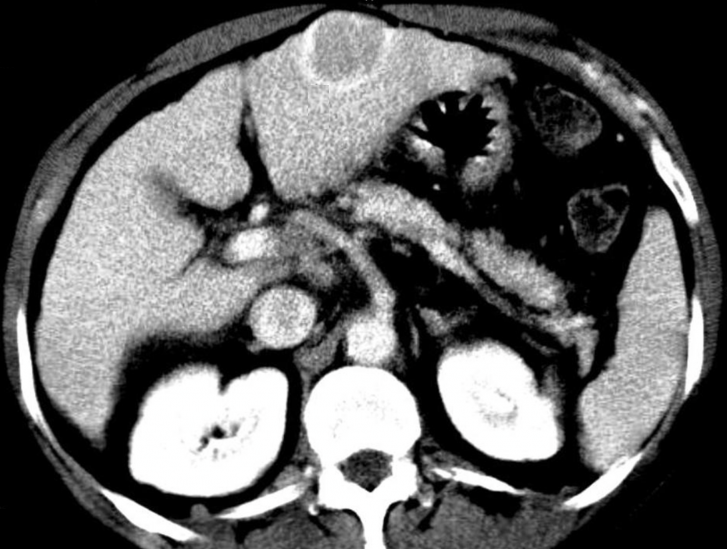
\includegraphics[width=0.8\linewidth]{tomo2}
  \caption{\texttt{tomo2}}
  \label{fig:sub1}
\end{subfigure}%
\begin{subfigure}{0.5\textwidth}
  \centering
  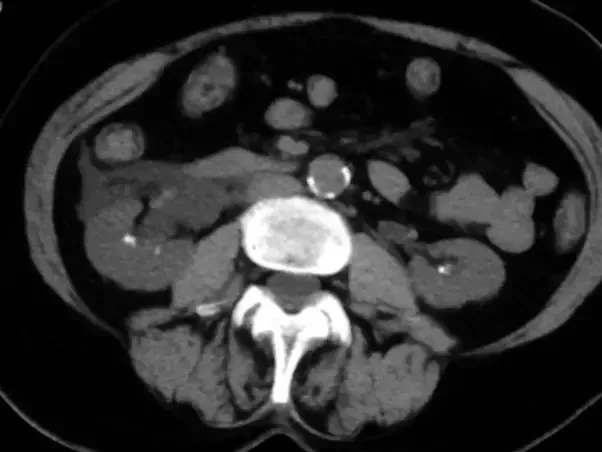
\includegraphics[width=0.8\linewidth]{tomo3}
  \caption{\texttt{tomo3}}
  \label{fig:sub2}
\end{subfigure}
\caption{Imágenes de prueba \texttt{tomo2} y \texttt{tomo3}.}
\label{fig:tomo23}
\end{figure}

\end{frame}

\begin{frame}
\frametitle{Experimentación: tamaño de celda}

\begin{figure}[h]
\centering
\begin{tikzpicture}
\begin{axis}[
    title={PSNR en función del tamaño de celda},
    xlabel={Tamaño de celda},
    ylabel={PSNR},
    xmin=10, xmax=20,
    ymin=14, ymax=23,
    xtick={10,11,12,13,14,15,16,17,18,19,20},
    ytick={14,15,16,17,18,19,20,21,22,23},
    legend pos=north east,
    ymajorgrids=true,
    xmajorgrids=true,
    grid style=dashed,
]

\addplot[
    color=blue,
    mark=*,
    style=dashed,
    ]
    coordinates {
    (20,14.2203)
    (19,14.4431)
    (18,14.584)
    (17,14.9159)
    (16,15.1494)
    (15,15.5134)
    (14,15.7002)
    (13,15.9758)
    (12,16.466)
    (11,16.8652)
    (10,17.2959)
    };
    \addlegendentry{\texttt{tomo2.csv}}

\addplot[
    color=red,
    mark=*,
    style=dashed,
    ]
    coordinates {
    (10,22.4565)
    (11,22.1921)
    (12,21.7393)
    (13,21.4325)
    (14,20.7527)
    (15,20.4585)
    (16,20.4911)
    (17,20.2983)
    (18,19.7594)
    (19,19.6317)
    (20,19.6563)
    };
    \addlegendentry{\texttt{tomo3.csv}}

\end{axis}
\end{tikzpicture}
\caption{PSNR en función del tamaño de celda, para las imágenes \texttt{tomo2.csv} y \texttt{tomo3.csv}. Nivel de ruido 0.0, 20000 rayos aleatorios.}
\label{fig:psnr_vs_celda_1}
\end{figure}


\end{frame}

\begin{frame}
\frametitle{Experimentación: tamaño de celda}

\begin{figure}[h]
\centering
\begin{tikzpicture}
\begin{axis}[
    title={$\kappa(D^tD)$ en función del tamaño de celda},
    xlabel={Tamaño de celda},
    ylabel={$\kappa(D^tD)$},
    xmin=10, xmax=20,
    ymin=0, ymax=30000,
    xtick={10,11,12,13,14,15,16,17,18,19,20},
    % ytick={0,1000,2000,3000,4000,5000,6000,7000},
    ytick={0,5000,10000,15000,20000,25000,30000},
    legend pos=north west,
    ymajorgrids=true,
    xmajorgrids=true,
    grid style=dashed,
]
 
\addplot[
    color=blue,
    mark=*,
    style=dashed,
    ]
    coordinates {
    (10,972.361)
    (11,721.499)
    (12,547.52)
    (13,6033.76)
    (14,6765.81)
    (15,383.894)
    (16,2051.95)
    (17,2258.71)
    (18,482.504)
    (19,218.039)
    (20,565.192)
    };
    \addlegendentry{\texttt{tomo2.csv}}

\addplot[
    color=red,
    mark=*,
    style=dashed,
    ]
    coordinates {
    (10,11483.7)
    (11,5439.17)
    (12,407.068)
    (13,277.723)
    (14,2690.57)
    (15,21570)
    (16,3345.09)
    (17,283.28)
    (18,29161.6)
    (19,133.389)
    (20,221.452)
    };
    \addlegendentry{\texttt{tomo3.csv}}
    
    
\end{axis}
\end{tikzpicture}
\caption{$\kappa(D^tD)$ en función del tamaño de celda, para las imágenes \texttt{tomo2.csv} y \texttt{tomo3.csv}. Nivel de ruido 0.0, 20000 rayos 
aleatorios.}
\label{fig:ncond_vs_celda_1}
\end{figure}

\end{frame}

\begin{frame}
\frametitle{Experimentación: tamaño de celda}

\begin{figure}
\centering

\begin{subfigure}{0.4\linewidth}
  \centering
  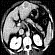
\includegraphics[width=0.6\linewidth]{celdas/tomo2-10-0}
  \caption{Tamaño de celda 10}
\end{subfigure}%
\begin{subfigure}{0.4\linewidth}
  \centering
  
\includegraphics[width=0.6\linewidth]{celdas/tomo2-13-0}
  \caption{Tamaño de celda 13}
\end{subfigure}
\begin{subfigure}{0.4\linewidth}
  \centering
  
\includegraphics[width=0.6\linewidth]{celdas/tomo2-17-0}
  \caption{Tamaño de celda 17}
\end{subfigure}%
\begin{subfigure}{0.4\linewidth}
  \centering
  
\includegraphics[width=0.6\linewidth]{celdas/tomo2-20-0}
  \caption{Tamaño de celda 20}
\end{subfigure}%

\caption{Imágen \texttt{tomo2.csv} reconstruida con diferentes tamaños de celda, nivel de ruido 0.0 y 20000 rayos aleatorios.}
\label{fig:muestras_celdas}
\end{figure}

\end{frame}

\begin{frame}
\frametitle{Experimentación: tamaño de celda}

\begin{figure}
\centering

\begin{subfigure}{0.4\linewidth}
  \centering
  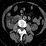
\includegraphics[width=0.6\linewidth]{celdas/tomo3-10-0}
  \caption{Tamaño de celda 10}
  \label{fig:muestras_celdas_tomo3_10}
\end{subfigure}%
\begin{subfigure}{0.4\linewidth}
  \centering
  
\includegraphics[width=0.6\linewidth]{celdas/tomo3-13-0}
  \caption{Tamaño de celda 13}
\end{subfigure}
\begin{subfigure}{0.4\linewidth}
  \centering
  
\includegraphics[width=0.6\linewidth]{celdas/tomo3-17-0}
  \caption{Tamaño de celda 17}
\end{subfigure}%
\begin{subfigure}{0.4\linewidth}
  \centering
  
\includegraphics[width=0.6\linewidth]{celdas/tomo3-20-0}
  \caption{Tamaño de celda 20}
\end{subfigure}%

\caption{Imágen \texttt{tomo3.csv} reconstruida con diferentes tamaños de celda, nivel de ruido 0.0 y 20000 rayos aleatorios.}
\label{fig:muestras_celdas}
\end{figure}

\end{frame}

\begin{frame}
\frametitle{Rayos verticales, horizontales y diagonales}
Se generan todos los rayos posibles que sean horizontales, verticales y diagonales con pendiente 1.
\begin{figure}
\centering
\begin{tikzpicture}[scale = 0.4]
% \draw [help lines] (0,0) grid (10,10);
\draw [thick] (0,0) rectangle (10,10);

\draw [ultra thin] (0,0.5) -- (10,0.5);
\draw [ultra thin] (0,1.5) -- (10,1.5);
\draw [ultra thin] (0,2.5) -- (10,2.5);
\draw [ultra thin] (0,3.5) -- (10,3.5);
\draw [ultra thin] (0,4.5) -- (10,4.5);
\draw [ultra thin] (0,5.5) -- (10,5.5);
\draw [ultra thin] (0,6.5) -- (10,6.5);
\draw [ultra thin] (0,7.5) -- (10,7.5);
\draw [ultra thin] (0,8.5) -- (10,8.5);
\draw [ultra thin] (0,9.5) -- (10,9.5);

\draw [ultra thin] (0.5,0) -- (0.5,10);
\draw [ultra thin] (1.5,0) -- (1.5,10);
\draw [ultra thin] (2.5,0) -- (2.5,10);
\draw [ultra thin] (3.5,0) -- (3.5,10);
\draw [ultra thin] (4.5,0) -- (4.5,10);
\draw [ultra thin] (5.5,0) -- (5.5,10);
\draw [ultra thin] (6.5,0) -- (6.5,10);
\draw [ultra thin] (7.5,0) -- (7.5,10);
\draw [ultra thin] (8.5,0) -- (8.5,10);
\draw [ultra thin] (9.5,0) -- (9.5,10);

\draw [ultra thin] (8,0) -- (10,2);
\draw [ultra thin] (7,0) -- (10,3);
\draw [ultra thin] (6,0) -- (10,4);
\draw [ultra thin] (5,0) -- (10,5);
\draw [ultra thin] (4,0) -- (10,6);
\draw [ultra thin] (3,0) -- (10,7);
\draw [ultra thin] (2,0) -- (10,8);
\draw [ultra thin] (1,0) -- (10,9);
\draw [ultra thin] (0,0) -- (10,10);
\draw [ultra thin] (0,1) -- (9,10);
\draw [ultra thin] (0,2) -- (8,10);
\draw [ultra thin] (0,3) -- (7,10);
\draw [ultra thin] (0,4) -- (6,10);
\draw [ultra thin] (0,5) -- (5,10);
\draw [ultra thin] (0,6) -- (4,10);
\draw [ultra thin] (0,7) -- (3,10);
\draw [ultra thin] (0,8) -- (2,10);

\draw [ultra thin] (0,2) -- (2,0);
\draw [ultra thin] (0,3) -- (3,0);
\draw [ultra thin] (0,4) -- (4,0);
\draw [ultra thin] (0,5) -- (5,0);
\draw [ultra thin] (0,6) -- (6,0);
\draw [ultra thin] (0,7) -- (7,0);
\draw [ultra thin] (0,8) -- (8,0);
\draw [ultra thin] (0,9) -- (9,0);
\draw [ultra thin] (0,10) -- (10,0);
\draw [ultra thin] (1,10) -- (10,1);
\draw [ultra thin] (2,10) -- (10,2);
\draw [ultra thin] (3,10) -- (10,3);
\draw [ultra thin] (4,10) -- (10,4);
\draw [ultra thin] (5,10) -- (10,5);
\draw [ultra thin] (6,10) -- (10,6);
\draw [ultra thin] (7,10) -- (10,7);
\draw [ultra thin] (8,10) -- (10,8);

\end{tikzpicture}
\end{figure}
\end{frame}

\begin{frame}
\frametitle{Experimentando: rayos verticales, horizontales y diagonales}

\begin{figure}
\centering
\begin{subfigure}{0.5\textwidth}
  \centering
  
\includegraphics[width=0.6\linewidth]{rayos/phantom-vhd}
  \caption{\texttt{phantom.csv}, con tamaño de celda 8}
\end{subfigure}%
\begin{subfigure}{0.5\textwidth}
  \centering
  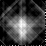
\includegraphics[width=0.6\linewidth]{rayos/tomo3-vhd}
  \caption{\texttt{tomo3.csv}, con tamaño de celda 10}
\end{subfigure}
\caption{Imágenes \texttt{phantom.csv} y \texttt{tomo3.csv} reconstruidas con rayos horizontales, verticales y diagonales. Nivel de ruido 0.0.}
\label{fig:muestras_vhd}
\end{figure}

\end{frame}

\begin{frame}
\frametitle{Experimentando: rayos verticales, horizontales y diagonales}

\begin{itemize}
\item \texttt{phantom.csv}:
\begin{itemize}
\item PSNR: 15.2316
\item 183 de 1024 autovalores de $D^tD$ calculados.
\item Chequeado con Numpy: $D^tD$ singular.%($1530 \times 1024$).
\end{itemize}
\item \texttt{tomo3.csv}:
\begin{itemize}
\item PSNR: 17.0948
\item 283 de 2116 autovalores de $D^tD$ calculados.
\item Chequeado con Numpy: $D^tD$ singular.%($2706 \times 2116$).
\end{itemize}
\end{itemize}

\end{frame}

\begin{frame}
\frametitle{Rayos que barren la imagen}
Consiste en pararse en cada una de las esquinas y generar rayos que vayan a todos los píxeles de los bordes no adyacentes.

\begin{figure}
\begin{tikzpicture}[scale=0.4]
\draw [thick] (0,0) rectangle (10,10);

\draw [ultra thin] (0,0) -- (1,10);
\draw [ultra thin] (0,0) -- (2,10);
\draw [ultra thin] (0,0) -- (3,10);
\draw [ultra thin] (0,0) -- (4,10);
\draw [ultra thin] (0,0) -- (5,10);
\draw [ultra thin] (0,0) -- (6,10);
\draw [ultra thin] (0,0) -- (7,10);
\draw [ultra thin] (0,0) -- (8,10);
\draw [ultra thin] (0,0) -- (9,10);
\draw [ultra thin] (0,0) -- (10,10);
\draw [ultra thin] (0,0) -- (10,9);
\draw [ultra thin] (0,0) -- (10,8);
\draw [ultra thin] (0,0) -- (10,7);
\draw [ultra thin] (0,0) -- (10,6);
\draw [ultra thin] (0,0) -- (10,5);
\draw [ultra thin] (0,0) -- (10,4);
\draw [ultra thin] (0,0) -- (10,3);
\draw [ultra thin] (0,0) -- (10,2);
\draw [ultra thin] (0,0) -- (10,1);

\draw [ultra thin] (10,0) -- (10,10);
\draw [ultra thin] (10,0) -- (9,10);
\draw [ultra thin] (10,0) -- (8,10);
\draw [ultra thin] (10,0) -- (7,10);
\draw [ultra thin] (10,0) -- (6,10);
\draw [ultra thin] (10,0) -- (5,10);
\draw [ultra thin] (10,0) -- (4,10);
\draw [ultra thin] (10,0) -- (3,10);
\draw [ultra thin] (10,0) -- (2,10);
\draw [ultra thin] (10,0) -- (1,10);
\draw [ultra thin] (10,0) -- (0,10);
\draw [ultra thin] (10,0) -- (0,9);
\draw [ultra thin] (10,0) -- (0,8);
\draw [ultra thin] (10,0) -- (0,7);
\draw [ultra thin] (10,0) -- (0,6);
\draw [ultra thin] (10,0) -- (0,5);
\draw [ultra thin] (10,0) -- (0,4);
\draw [ultra thin] (10,0) -- (0,3);
\draw [ultra thin] (10,0) -- (0,2);
\draw [ultra thin] (10,0) -- (0,1);
\draw [ultra thin] (10,0) -- (0,0);

\draw [ultra thin] (0,10) -- (10,10);
\draw [ultra thin] (0,10) -- (10,9);
\draw [ultra thin] (0,10) -- (10,8);
\draw [ultra thin] (0,10) -- (10,7);
\draw [ultra thin] (0,10) -- (10,6);
\draw [ultra thin] (0,10) -- (10,5);
\draw [ultra thin] (0,10) -- (10,4);
\draw [ultra thin] (0,10) -- (10,3);
\draw [ultra thin] (0,10) -- (10,2);
\draw [ultra thin] (0,10) -- (10,1);
\draw [ultra thin] (0,10) -- (10,0);
\draw [ultra thin] (0,10) -- (9,0);
\draw [ultra thin] (0,10) -- (8,0);
\draw [ultra thin] (0,10) -- (7,0);
\draw [ultra thin] (0,10) -- (6,0);
\draw [ultra thin] (0,10) -- (5,0);
\draw [ultra thin] (0,10) -- (4,0);
\draw [ultra thin] (0,10) -- (3,0);
\draw [ultra thin] (0,10) -- (2,0);
\draw [ultra thin] (0,10) -- (1,0);
\draw [ultra thin] (0,10) -- (0,0);

\draw [ultra thin] (10,10) -- (0,10);
\draw [ultra thin] (10,10) -- (0,9);
\draw [ultra thin] (10,10) -- (0,8);
\draw [ultra thin] (10,10) -- (0,7);
\draw [ultra thin] (10,10) -- (0,6);
\draw [ultra thin] (10,10) -- (0,5);
\draw [ultra thin] (10,10) -- (0,4);
\draw [ultra thin] (10,10) -- (0,3);
\draw [ultra thin] (10,10) -- (0,2);
\draw [ultra thin] (10,10) -- (0,1);
\draw [ultra thin] (10,10) -- (0,0);
\draw [ultra thin] (10,10) -- (1,0);
\draw [ultra thin] (10,10) -- (2,0);
\draw [ultra thin] (10,10) -- (3,0);
\draw [ultra thin] (10,10) -- (4,0);
\draw [ultra thin] (10,10) -- (5,0);
\draw [ultra thin] (10,10) -- (6,0);
\draw [ultra thin] (10,10) -- (7,0);
\draw [ultra thin] (10,10) -- (8,0);
\draw [ultra thin] (10,10) -- (9,0);
\draw [ultra thin] (10,10) -- (10,0);
\end{tikzpicture}
\end{figure}
\end{frame}

\begin{frame}
\frametitle{Experimentando: rayos que barren la imagen}

\begin{figure}
\centering
\begin{subfigure}{0.5\textwidth}
  \centering
  
\includegraphics[width=0.6\linewidth]{rayos/phantom-barrido}
  \caption{\texttt{phantom.csv}, con tamaño de celda 8}
\end{subfigure}%
\begin{subfigure}{0.5\textwidth}
  \centering
  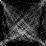
\includegraphics[width=0.6\linewidth]{rayos/tomo3-barrido}
  \caption{\texttt{tomo3.csv}, con tamaño de celda 10}
\end{subfigure}
\caption{Imágenes \texttt{phantom.csv} y \texttt{tomo3.csv} reconstruidas con rayos que barren la imagen desde las cuatro esquinas. Nivel de 
ruido 0.0.}
\label{fig:muestras_barrido}
\end{figure}

\end{frame}

\begin{frame}
\frametitle{Experimentando: rayos que barren la imagen}

\begin{itemize}
\item \texttt{phantom.csv}:
\begin{itemize}
\item PSNR: 12.4005
\item 790 de 1024 autovalores de $D^tD$ calculados.
\item Chequeado con Numpy: $\kappa(D^tD) = 1578918$.
\end{itemize}
\item \texttt{tomo3.csv}:
\begin{itemize}
\item PSNR: 13.9602
\item 1088 de 2116 autovalores de $D^tD$ calculados.
\item Chequeado con Numpy: $\kappa(D^tD) = 6470105$.
\end{itemize}
\end{itemize}

\end{frame}

\begin{frame}
\frametitle{Rayos aleatorios}
Dada una cantidad de rayos deseada $m$. Se genera cada rayo de la siguiente manera:
\begin{enumerate}
	\item<1-> [1.] Se elige la trayectoria del rayo en términos de en qué borde partirá el rayo y hasta cuál llegará.
	\item<2-> [2.] Se elige un punto de cada borde elegido, los cuales determinarán el rayo.
\end{enumerate}
\end{frame}

\begin{frame}
\frametitle{Experimentando: Cantidad de rayos aleatorios}
\begin{figure}[h]
\centering
\begin{tikzpicture}
\begin{axis}[
    title={PSNR en función de la cantidad de rayos aleatorios},
    xlabel={Cantidad de rayos aleatorios},
    ylabel={PSNR},
    xmin=0, xmax=7000,
    ymin=8, ymax=22,
    xtick={0,1000,2000,3000,4000,5000,6000,7000},
    ytick={8,10,12,14,16,18,20,22},
    legend pos=south east,
    ymajorgrids=true,
    % xmajorgrids=true,
    grid style=dashed,
]
 
\addplot[
    color=blue,
    % mark=*,
    % style=dashed,
    ]
    coordinates {
    (1444,15.7564)
    (2000,15.9915)
    (2500,17.2767)
    (3000,19.0018)
    (3500,19.9412)
    (4000,20.1737)
    (4500,20.6685)
    (5000,20.8324)
    (5500,21.0253)
    (6000,21.1197)
    (6500,21.1539)
    (7000,21.2395)
    };
    \addlegendentry{\texttt{tomo3.csv}}

\addplot[
    color=red,
    % mark=*,
    % style=dashed,
    ]
    coordinates {
    (676,8.41618)
    (1000,11.3252)
    (1500,15.016 )
    (2000,15.6017)
    (2500,16.1013)
    (3000,16.2221)
    (3500,16.3056)
    (4000,16.3317)
    (4500,16.3707)
    (5000,16.4363)
    (5500,16.4824)
    (6000,16.4942)
    (6500,16.5166)
    (7000,16.5248)
    };
    \addlegendentry{\texttt{phantom.csv}}

\end{axis}
\end{tikzpicture}
\caption{PSNR en función de cantidad de rayos aleatorios, para las imágenes \texttt{tomo3.csv} y \texttt{phantom.csv}, tamaños de celda 
12 y 10 respectivamente, y nivel de ruido 0.0.}
\label{fig:psnr_vs_aleats}
\end{figure}
\end{frame}

\begin{frame}
\frametitle{Experimentando: Cantidad de rayos aleatorios}

\begin{figure}[h]
\centering
\begin{tikzpicture}
\begin{axis}[
    title={$\kappa(D^tD)$ en función de cant de rayos aleatorios},
    xlabel={Cantidad de rayos aleatorios},
    ylabel={$\kappa(D^tD)$},
    xmin=0, xmax=7000,
    ymin=0, ymax=36000,
    xtick={0,1000,2000,3000,4000,5000,6000,7000},
    ytick={0,5000,10000,15000,20000,25000,30000,35000},
    legend pos=north east,
    ymajorgrids=true,
    % xmajorgrids=true,
    grid style=dashed,
]
 
\addplot[
    color=blue,
    % mark=*,
    % style=dashed,
    ]
    coordinates {
    (2500,35281.5)
    (3000,22873)
    (3500,4247.11)
    (4000,2171.75)
    (4500,1884.09)
    (5000,1443.61)
    (5500,1115.55)
    (6000,1155.68)
    (6500,775.142)
    (7000,707.507)
    };
    \addlegendentry{\texttt{tomo3.csv}}

\addplot[
    color=red,
    % mark=*,
    % style=dashed,
    ]
    coordinates {
    (1500,11736.9)
    (2000,8422.15)
    (2500,964.307)
    (3000,550.485)
    (3500,442.103)
    (4000,341.59)
    (4500,317.157)
    (5000,300.344)
    (5500,290.834)
    (6000,283.758)
    (6500,276.984)
    (7000,265.96)
    };
    \addlegendentry{\texttt{phantom.csv}}

\end{axis}
\end{tikzpicture}
\caption{$\kappa(D^tD)$ en función de cantidad de rayos aleatorios, para las imágenes \texttt{tomo3.csv} y \texttt{phantom.csv}, tamaños de celda 
12 y 10 respectivamente, y nivel de ruido 0.0.}
\label{fig:ncond_vs_aleats}
\end{figure}
\end{frame}

\begin{frame}
\frametitle{Experimentando: Cantidad de rayos aleatorios}
\begin{figure}
\centering
\begin{subfigure}{0.4\linewidth}
  \centering
  
\includegraphics[width=0.6\linewidth]{rayos/tomo3-aleat1444}
  \caption{1444 rayos aleatorios ($D$ resulta cuadrada).}
\end{subfigure}%
\begin{subfigure}{0.4\linewidth}
  \centering
  
\includegraphics[width=0.6\linewidth]{rayos/tomo3-aleat2500}
  \caption{2500 rayos aleatorios.}
\end{subfigure}
\begin{subfigure}{0.4\linewidth}
  \centering
  
\includegraphics[width=0.6\linewidth]{rayos/tomo3-aleat4000}
  \caption{4000 rayos aleatorios.}
\end{subfigure}%
\begin{subfigure}{0.4\linewidth}
  \centering
  
\includegraphics[width=0.6\linewidth]{rayos/tomo3-aleat7000}
  \caption{7000 rayos aleatorios.}
\end{subfigure}%
\caption{Imagen \texttt{tomo3.csv} reconstruida con tamaño de celda 12, nivel de ruido 0.0. Se 
muestran resultados para diferentes cantidades de rayos aleatorios.}
\label{fig:muestras_aleat}
\end{figure}
\end{frame}

\begin{frame}
\frametitle{Experimentando: Cantidad de rayos aleatorios}

\begin{figure}
\centering
\begin{subfigure}{0.4\linewidth}
  \centering
  
\includegraphics[width=0.6\linewidth]{rayos/phantom-aleat676}
  \caption{676 rayos aleatorios ($D$ resulta cuadrada).}
\end{subfigure}%
\begin{subfigure}{0.4\linewidth}
  \centering
  
\includegraphics[width=0.6\linewidth]{rayos/phantom-aleat1500}
  \caption{1500 rayos aleatorios.}
\end{subfigure}
\begin{subfigure}{0.4\linewidth}
  \centering
  
\includegraphics[width=0.6\linewidth]{rayos/phantom-aleat4000}
  \caption{4000 rayos aleatorios.}
\end{subfigure}%
\begin{subfigure}{0.4\linewidth}
  \centering
  
\includegraphics[width=0.6\linewidth]{rayos/phantom-aleat7000}
  \caption{7000 rayos aleatorios.}
\end{subfigure}%

\caption{Imagen \texttt{phantom.csv} reconstruida con tamaño de celda 10, nivel de ruido 0.0. Se 
muestran resultados para diferentes cantidades de rayos aleatorios.}
\label{fig:muestras_aleat}
\end{figure}
\end{frame}

\begin{frame}
\frametitle{Metodo $"$completo$"$}
Se generan todos los rayos posibles que pasen por dos píxeles que estén en bordes opuestos de la imagen.
\begin{figure}
\begin{tikzpicture}[scale=0.4]
\draw [thick] (0,0) rectangle (10,10);

\draw [ultra thin] (0,0) -- (0,10);
\draw [ultra thin] (0,0) -- (1,10);
\draw [ultra thin] (0,0) -- (2,10);
\draw [ultra thin] (0,0) -- (3,10);
\draw [ultra thin] (0,0) -- (4,10);
\draw [ultra thin] (0,0) -- (5,10);
\draw [ultra thin] (0,0) -- (6,10);
\draw [ultra thin] (0,0) -- (7,10);
\draw [ultra thin] (0,0) -- (8,10);
\draw [ultra thin] (0,0) -- (9,10);
\draw [ultra thin] (0,0) -- (10,10);

\draw [ultra thin] (1,0) -- (0,10);
\draw [ultra thin] (1,0) -- (1,10);
\draw [ultra thin] (1,0) -- (2,10);
\draw [ultra thin] (1,0) -- (3,10);
\draw [ultra thin] (1,0) -- (4,10);
\draw [ultra thin] (1,0) -- (5,10);
\draw [ultra thin] (1,0) -- (6,10);
\draw [ultra thin] (1,0) -- (7,10);
\draw [ultra thin] (1,0) -- (8,10);
\draw [ultra thin] (1,0) -- (9,10);
\draw [ultra thin] (1,0) -- (10,10);

\draw [ultra thin] (2,0) -- (0,10);
\draw [ultra thin] (2,0) -- (1,10);
\draw [ultra thin] (2,0) -- (2,10);
\draw [ultra thin] (2,0) -- (3,10);
\draw [ultra thin] (2,0) -- (4,10);
\draw [ultra thin] (2,0) -- (5,10);
\draw [ultra thin] (2,0) -- (6,10);
\draw [ultra thin] (2,0) -- (7,10);
\draw [ultra thin] (2,0) -- (8,10);
\draw [ultra thin] (2,0) -- (9,10);
\draw [ultra thin] (2,0) -- (10,10);

\draw [ultra thin] (3,0) -- (0,10);
\draw [ultra thin] (3,0) -- (1,10);
\draw [ultra thin] (3,0) -- (2,10);
\draw [ultra thin] (3,0) -- (3,10);
\draw [ultra thin] (3,0) -- (4,10);
\draw [ultra thin] (3,0) -- (5,10);
\draw [ultra thin] (3,0) -- (6,10);
\draw [ultra thin] (3,0) -- (7,10);
\draw [ultra thin] (3,0) -- (8,10);
\draw [ultra thin] (3,0) -- (9,10);
\draw [ultra thin] (3,0) -- (10,10);

\draw [ultra thin] (4,0) -- (0,10);
\draw [ultra thin] (4,0) -- (1,10);
\draw [ultra thin] (4,0) -- (2,10);
\draw [ultra thin] (4,0) -- (3,10);
\draw [ultra thin] (4,0) -- (4,10);
\draw [ultra thin] (4,0) -- (5,10);
\draw [ultra thin] (4,0) -- (6,10);
\draw [ultra thin] (4,0) -- (7,10);
\draw [ultra thin] (4,0) -- (8,10);
\draw [ultra thin] (4,0) -- (9,10);
\draw [ultra thin] (4,0) -- (10,10);

\draw [ultra thin] (5,0) -- (0,10);
\draw [ultra thin] (5,0) -- (1,10);
\draw [ultra thin] (5,0) -- (2,10);
\draw [ultra thin] (5,0) -- (3,10);
\draw [ultra thin] (5,0) -- (4,10);
\draw [ultra thin] (5,0) -- (5,10);
\draw [ultra thin] (5,0) -- (6,10);
\draw [ultra thin] (5,0) -- (7,10);
\draw [ultra thin] (5,0) -- (8,10);
\draw [ultra thin] (5,0) -- (9,10);
\draw [ultra thin] (5,0) -- (10,10);

\draw [ultra thin] (6,0) -- (0,10);
\draw [ultra thin] (6,0) -- (1,10);
\draw [ultra thin] (6,0) -- (2,10);
\draw [ultra thin] (6,0) -- (3,10);
\draw [ultra thin] (6,0) -- (4,10);
\draw [ultra thin] (6,0) -- (5,10);
\draw [ultra thin] (6,0) -- (6,10);
\draw [ultra thin] (6,0) -- (7,10);
\draw [ultra thin] (6,0) -- (8,10);
\draw [ultra thin] (6,0) -- (9,10);
\draw [ultra thin] (6,0) -- (10,10);

\draw [ultra thin] (7,0) -- (0,10);
\draw [ultra thin] (7,0) -- (1,10);
\draw [ultra thin] (7,0) -- (2,10);
\draw [ultra thin] (7,0) -- (3,10);
\draw [ultra thin] (7,0) -- (4,10);
\draw [ultra thin] (7,0) -- (5,10);
\draw [ultra thin] (7,0) -- (6,10);
\draw [ultra thin] (7,0) -- (7,10);
\draw [ultra thin] (7,0) -- (8,10);
\draw [ultra thin] (7,0) -- (9,10);
\draw [ultra thin] (7,0) -- (10,10);

\draw [ultra thin] (8,0) -- (0,10);
\draw [ultra thin] (8,0) -- (1,10);
\draw [ultra thin] (8,0) -- (2,10);
\draw [ultra thin] (8,0) -- (3,10);
\draw [ultra thin] (8,0) -- (4,10);
\draw [ultra thin] (8,0) -- (5,10);
\draw [ultra thin] (8,0) -- (6,10);
\draw [ultra thin] (8,0) -- (7,10);
\draw [ultra thin] (8,0) -- (8,10);
\draw [ultra thin] (8,0) -- (9,10);
\draw [ultra thin] (8,0) -- (10,10);

\draw [ultra thin] (9,0) -- (0,10);
\draw [ultra thin] (9,0) -- (1,10);
\draw [ultra thin] (9,0) -- (2,10);
\draw [ultra thin] (9,0) -- (3,10);
\draw [ultra thin] (9,0) -- (4,10);
\draw [ultra thin] (9,0) -- (5,10);
\draw [ultra thin] (9,0) -- (6,10);
\draw [ultra thin] (9,0) -- (7,10);
\draw [ultra thin] (9,0) -- (8,10);
\draw [ultra thin] (9,0) -- (9,10);
\draw [ultra thin] (9,0) -- (10,10);

\draw [ultra thin] (10,0) -- (0,10);
\draw [ultra thin] (10,0) -- (1,10);
\draw [ultra thin] (10,0) -- (2,10);
\draw [ultra thin] (10,0) -- (3,10);
\draw [ultra thin] (10,0) -- (4,10);
\draw [ultra thin] (10,0) -- (5,10);
\draw [ultra thin] (10,0) -- (6,10);
\draw [ultra thin] (10,0) -- (7,10);
\draw [ultra thin] (10,0) -- (8,10);
\draw [ultra thin] (10,0) -- (9,10);
\draw [ultra thin] (10,0) -- (10,10);

\draw [ultra thin] (0,0) -- (10,0);
\draw [ultra thin] (0,0) -- (10,1);
\draw [ultra thin] (0,0) -- (10,2);
\draw [ultra thin] (0,0) -- (10,3);
\draw [ultra thin] (0,0) -- (10,4);
\draw [ultra thin] (0,0) -- (10,5);
\draw [ultra thin] (0,0) -- (10,6);
\draw [ultra thin] (0,0) -- (10,7);
\draw [ultra thin] (0,0) -- (10,8);
\draw [ultra thin] (0,0) -- (10,9);
\draw [ultra thin] (0,0) -- (10,10);

\draw [ultra thin] (0,1) -- (10,0);
\draw [ultra thin] (0,1) -- (10,1);
\draw [ultra thin] (0,1) -- (10,2);
\draw [ultra thin] (0,1) -- (10,3);
\draw [ultra thin] (0,1) -- (10,4);
\draw [ultra thin] (0,1) -- (10,5);
\draw [ultra thin] (0,1) -- (10,6);
\draw [ultra thin] (0,1) -- (10,7);
\draw [ultra thin] (0,1) -- (10,8);
\draw [ultra thin] (0,1) -- (10,9);
\draw [ultra thin] (0,1) -- (10,10);

\draw [ultra thin] (0,2) -- (10,0);
\draw [ultra thin] (0,2) -- (10,1);
\draw [ultra thin] (0,2) -- (10,2);
\draw [ultra thin] (0,2) -- (10,3);
\draw [ultra thin] (0,2) -- (10,4);
\draw [ultra thin] (0,2) -- (10,5);
\draw [ultra thin] (0,2) -- (10,6);
\draw [ultra thin] (0,2) -- (10,7);
\draw [ultra thin] (0,2) -- (10,8);
\draw [ultra thin] (0,2) -- (10,9);
\draw [ultra thin] (0,2) -- (10,10);

\draw [ultra thin] (0,3) -- (10,0);
\draw [ultra thin] (0,3) -- (10,1);
\draw [ultra thin] (0,3) -- (10,2);
\draw [ultra thin] (0,3) -- (10,3);
\draw [ultra thin] (0,3) -- (10,4);
\draw [ultra thin] (0,3) -- (10,5);
\draw [ultra thin] (0,3) -- (10,6);
\draw [ultra thin] (0,3) -- (10,7);
\draw [ultra thin] (0,3) -- (10,8);
\draw [ultra thin] (0,3) -- (10,9);
\draw [ultra thin] (0,3) -- (10,10);

\draw [ultra thin] (0,4) -- (10,0);
\draw [ultra thin] (0,4) -- (10,1);
\draw [ultra thin] (0,4) -- (10,2);
\draw [ultra thin] (0,4) -- (10,3);
\draw [ultra thin] (0,4) -- (10,4);
\draw [ultra thin] (0,4) -- (10,5);
\draw [ultra thin] (0,4) -- (10,6);
\draw [ultra thin] (0,4) -- (10,7);
\draw [ultra thin] (0,4) -- (10,8);
\draw [ultra thin] (0,4) -- (10,9);
\draw [ultra thin] (0,4) -- (10,10);

\draw [ultra thin] (0,5) -- (10,0);
\draw [ultra thin] (0,5) -- (10,1);
\draw [ultra thin] (0,5) -- (10,2);
\draw [ultra thin] (0,5) -- (10,3);
\draw [ultra thin] (0,5) -- (10,4);
\draw [ultra thin] (0,5) -- (10,5);
\draw [ultra thin] (0,5) -- (10,6);
\draw [ultra thin] (0,5) -- (10,7);
\draw [ultra thin] (0,5) -- (10,8);
\draw [ultra thin] (0,5) -- (10,9);
\draw [ultra thin] (0,5) -- (10,10);

\draw [ultra thin] (0,6) -- (10,0);
\draw [ultra thin] (0,6) -- (10,1);
\draw [ultra thin] (0,6) -- (10,2);
\draw [ultra thin] (0,6) -- (10,3);
\draw [ultra thin] (0,6) -- (10,4);
\draw [ultra thin] (0,6) -- (10,5);
\draw [ultra thin] (0,6) -- (10,6);
\draw [ultra thin] (0,6) -- (10,7);
\draw [ultra thin] (0,6) -- (10,8);
\draw [ultra thin] (0,6) -- (10,9);
\draw [ultra thin] (0,6) -- (10,10);

\draw [ultra thin] (0,7) -- (10,0);
\draw [ultra thin] (0,7) -- (10,1);
\draw [ultra thin] (0,7) -- (10,2);
\draw [ultra thin] (0,7) -- (10,3);
\draw [ultra thin] (0,7) -- (10,4);
\draw [ultra thin] (0,7) -- (10,5);
\draw [ultra thin] (0,7) -- (10,6);
\draw [ultra thin] (0,7) -- (10,7);
\draw [ultra thin] (0,7) -- (10,8);
\draw [ultra thin] (0,7) -- (10,9);
\draw [ultra thin] (0,7) -- (10,10);

\draw [ultra thin] (0,8) -- (10,0);
\draw [ultra thin] (0,8) -- (10,1);
\draw [ultra thin] (0,8) -- (10,2);
\draw [ultra thin] (0,8) -- (10,3);
\draw [ultra thin] (0,8) -- (10,4);
\draw [ultra thin] (0,8) -- (10,5);
\draw [ultra thin] (0,8) -- (10,6);
\draw [ultra thin] (0,8) -- (10,7);
\draw [ultra thin] (0,8) -- (10,8);
\draw [ultra thin] (0,8) -- (10,9);
\draw [ultra thin] (0,8) -- (10,10);

\draw [ultra thin] (0,9) -- (10,0);
\draw [ultra thin] (0,9) -- (10,1);
\draw [ultra thin] (0,9) -- (10,2);
\draw [ultra thin] (0,9) -- (10,3);
\draw [ultra thin] (0,9) -- (10,4);
\draw [ultra thin] (0,9) -- (10,5);
\draw [ultra thin] (0,9) -- (10,6);
\draw [ultra thin] (0,9) -- (10,7);
\draw [ultra thin] (0,9) -- (10,8);
\draw [ultra thin] (0,9) -- (10,9);
\draw [ultra thin] (0,9) -- (10,10);

\draw [ultra thin] (0,10) -- (10,0);
\draw [ultra thin] (0,10) -- (10,1);
\draw [ultra thin] (0,10) -- (10,2);
\draw [ultra thin] (0,10) -- (10,3);
\draw [ultra thin] (0,10) -- (10,4);
\draw [ultra thin] (0,10) -- (10,5);
\draw [ultra thin] (0,10) -- (10,6);
\draw [ultra thin] (0,10) -- (10,7);
\draw [ultra thin] (0,10) -- (10,8);
\draw [ultra thin] (0,10) -- (10,9);
\draw [ultra thin] (0,10) -- (10,10);

\end{tikzpicture}
\end{figure}

\end{frame}

\begin{frame}
\frametitle{Experimentando: método completo}

\begin{figure}
\centering
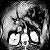
\includegraphics[width=0.3\linewidth]{rayos/tomo-completo}
\caption{Imagen \texttt{tomo.csv} reconstruida con el método ``completo'', tamaño de celda 2 y nivel de ruido 0.0.}
\label{fig:muestra_completo}
\end{figure}

\end{frame}

\begin{frame}
\frametitle{Experimentando: nivel de ruido}

\begin{figure}[h]
\centering
\begin{tikzpicture}
\begin{axis}[
    title={PSNR en función del nivel de ruido},
    xlabel={Nivel de ruido},
    ylabel={PSNR},
    xmin=0, xmax=20000,
    ymin=11, ymax=18,
    xtick={0,2000,4000,6000,8000,10000,12000,14000,16000,18000,20000},
    ytick={11,12,13,14,15,16,17,18},
    legend pos=south west,
    ymajorgrids=true,
    % xmajorgrids=true,
    grid style=dashed,
]
 
\addplot[
    color=blue,
    % mark=*,
    % style=dashed,
    ]
    coordinates {
    (0, 17.3091)
    (250,17.3067)
    (500,17.3023)
    (750,17.2877)
    (1000,17.2651)
    (1250,17.2518)
    (1500,17.2267)
    (1750,17.2191)
    (2000,17.1525)
    (2250,17.1179)
    (2500,17.0655)
    (2750,17.0334)
    (3000,16.96)
    (3250,16.8747)
    (3500,16.8909)
    (3750,16.8216)
    (4000,16.7531)
    (4250,16.7148)
    (4500,16.6147)
    (4750,16.529)
    (5000,16.4476)
    (5250,16.3861)
    (5500,16.3223)
    (5750,16.1855)
    (6000,16.0697)
    (6250,16.0754)
    (6500,15.9512)
    (6750,15.8443)
    (7000,15.8042)
    (7250,15.7652)
    (7500,15.6609)
    (7750,15.454)
    (8000,15.407)
    (8250,15.2654)
    (8500,15.1496)
    (8750,15.1083)
    (9000,15.0599)
    (9250,14.9569)
    (9500,14.8081)
    (9750,14.7154)
    (10000, 14.587)
    (10500, 14.5426)
    (11000, 14.2761)
    (11500, 14.1894)
    (12000, 14.0327)
    (12500, 13.8666)
    (13000, 13.6129)
    (13500, 13.5144)
    (14000, 13.2077)
    (14500, 13.1337)
    (15000, 12.9271)
    (15500, 12.7269)
    (16000, 12.5547)
    (16500, 12.5602)
    (17000, 12.1882)
    (17500, 12.1494)
    (18000, 11.9452)
    (18500, 11.6838)
    (19000, 11.7889)
    (19500, 11.5614)
    (20000, 11.4249)
    };
    \addlegendentry{\texttt{tomo2.csv}}

\end{axis}
\end{tikzpicture}
\caption{PSNR en función del nivel de ruido agregado a los tiempos de los rayos, para la imagen \texttt{tomo2.csv}, tamaño de celda 
10 con 20000 rayos aleatorios.}
\label{fig:psnr_vs_ruido}
\end{figure}

\end{frame}

\begin{frame}
\frametitle{Experimentando: nivel de ruido}

\begin{figure}
\centering
\begin{subfigure}{0.49\textwidth}
  \centering
  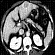
\includegraphics[width=0.6\linewidth]{ruido/tomo2-ruido0}
  \caption{Nivel de ruido: 0.}
\end{subfigure}
\begin{subfigure}{0.49\textwidth}
  \centering
  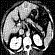
\includegraphics[width=0.6\linewidth]{ruido/tomo2-ruido4000}
  \caption{Nivel de ruido: 4000.}
\end{subfigure}
\caption{Imagen \texttt{tomo2.csv} reconstruida con tamaño de celda 10 y 20000 rayos aleatorios. Se 
muestran resultados para diferentes niveles de ruido.}
\label{fig:muestras_ruido}
\end{figure}

\end{frame}

\begin{frame}
\frametitle{Experimentando: nivel de ruido}

\begin{figure}
\centering
\begin{subfigure}{0.49\textwidth}
  \centering
  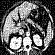
\includegraphics[width=0.6\linewidth]{ruido/tomo2-ruido8000}
  \caption{Nivel de ruido: 8000.}
\end{subfigure}
\begin{subfigure}{0.49\textwidth}
  \centering
  
\includegraphics[width=0.6\linewidth]{ruido/tomo2-ruido12000}
  \caption{Nivel de ruido: 12000.}
\end{subfigure}
\caption{Imagen \texttt{tomo2.csv} reconstruida con tamaño de celda 10 y 20000 rayos aleatorios. Se 
muestran resultados para diferentes niveles de ruido.}
\label{fig:muestras_ruido}
\end{figure}

\end{frame}

\begin{frame}
\frametitle{Experimentando: nivel de ruido}

\begin{figure}
\centering
\begin{subfigure}{0.49\textwidth}
  \centering
  
\includegraphics[width=0.6\linewidth]{ruido/tomo2-ruido16000}
  \caption{Nivel de ruido: 16000.}
\end{subfigure}
\begin{subfigure}{0.49\textwidth}
  \centering
  
\includegraphics[width=0.6\linewidth]{ruido/tomo2-ruido20000}
  \caption{Nivel de ruido: 20000.}
\end{subfigure}
\caption{Imagen \texttt{tomo2.csv} reconstruida con tamaño de celda 10 y 20000 rayos aleatorios. Se 
muestran resultados para diferentes niveles de ruido.}
\label{fig:muestras_ruido}
\end{figure}


\end{frame}

\begin{frame}
\frametitle{Conclusiones}
\begin{itemize}
\item<1-> La manera en la que se emiten los rayos es decisiva a la hora de evaluar qué tan buena fue la reconstrucción.
\item<2-> Un tamaño de celda más chico implica mejor calidad (pero es más costoso en tiempo).
\item<3-> La descomposición SVD es apropiada para hallar la solución de cuadrados mínimos. Pero es necesario contar con un método para obtener 
autovalores y autovectores eficazmente.
\item<4-> La aproximación de la solución mediante cuadrados mínimos es un método efectivo a la hora de reconstruir la imagen original.
\end{itemize}
\end{frame}

\begin{frame}
\frametitle{Posibles extensiones}
Algunos cambios que podrían hacerse son:
\begin{itemize}
\item<1-> Usar otro algoritmo para obtener autovalores y autovectores.
\item<2-> Usar las factorizaciones QR y Cholesky de $D^{t}D$, los métodos iterativos de Jacobi, Gauss-Seidel o la eliminación Gaussiana para resolver 
las ecuaciones normales.
\item<3-> Nuevos métodos de generación de rayos.
\end{itemize}

\end{frame}

\end{document}

